
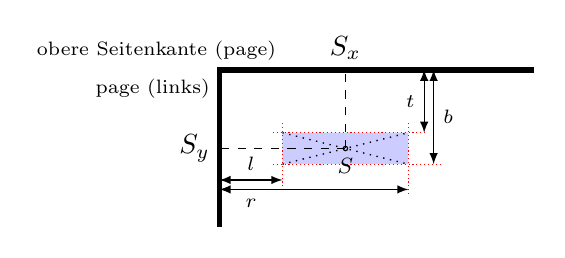
\begin{tikzpicture}[fill=blue!20, scale=0.4]

% Koordinaten/Beschriftungen
\draw[line width=2pt] (0,-5) -- (0,0) -- (10,0);
\draw (-2,0) node[anchor=south]{\scriptsize obere Seitenkante (\code{page})};
\draw (0,-0.6) node[anchor=east]{\scriptsize \code{page} (links)};

% Element
\fill (2,-2) -- (6,-2) -- (6,-3) -- (2,-3) -- (2,-2);

% Pfeile horizontal
\draw[>=latex,<->] (0,-3.5) -- (2, -3.5);
\draw[>=latex,<->] (0,-3.8) -- (6, -3.8);
\draw (1, -3.5) node[anchor=south]{{\scriptsize $l$}};
\draw (1, -3.8) node[anchor=north]{{\scriptsize $r$}};

% Pfeile vertikal
\draw[>=latex,<->] (6.5,0) -- (6.5, -2);
\draw[>=latex,<->] (6.8,0) -- (6.8, -3);
\draw (6.5, -1) node[anchor=east]{{\scriptsize $t$}};
\draw (6.8, -1.5) node[anchor=west]{{\scriptsize $b$}};

% Hilfslinien
\draw[red, densely dotted] (1.7,-2) -- (6.6,-2);
\draw[red, densely dotted] (1.7,-3) -- (7.1,-3);
\draw[red, densely dotted] (2,-1.7) -- (2,-3.7);
\draw[red, densely dotted] (6,-1.7) -- (6,-4);

% Diag
\draw (4,-2.5) circle (2pt);
\draw[dotted, line width=0.5pt] (2,-2) -- (6,-3);
\draw[dotted, line width=0.5pt] (2,-3) -- (6,-2);
\draw (4,-2.5) node[anchor=north]{{\footnotesize $S$}};

% Koordinaten
\draw[dashed] (4,-2.5) -- (4,0) node[anchor=south]{$S_x$};
\draw[dashed] (4,-2.5) -- (0,-2.5) node[anchor=east]{$S_y$};
\end{tikzpicture}
